% Options for packages loaded elsewhere
\PassOptionsToPackage{unicode}{hyperref}
\PassOptionsToPackage{hyphens}{url}
%
\documentclass[
  ignorenonframetext,
  aspectratio=169,
]{beamer}
\usepackage{pgfpages}
\setbeamertemplate{caption}[numbered]
\setbeamertemplate{caption label separator}{: }
\setbeamercolor{caption name}{fg=normal text.fg}
\beamertemplatenavigationsymbolshorizontal
% Prevent slide breaks in the middle of a paragraph
\widowpenalties 1 10000
\raggedbottom
\setbeamertemplate{part page}{
  \centering
  \begin{beamercolorbox}[sep=16pt,center]{part title}
    \usebeamerfont{part title}\insertpart\par
  \end{beamercolorbox}
}
\setbeamertemplate{section page}{
  \centering
  \begin{beamercolorbox}[sep=12pt,center]{part title}
    \usebeamerfont{section title}\insertsection\par
  \end{beamercolorbox}
}
\setbeamertemplate{subsection page}{
  \centering
  \begin{beamercolorbox}[sep=8pt,center]{part title}
    \usebeamerfont{subsection title}\insertsubsection\par
  \end{beamercolorbox}
}
\AtBeginPart{
  \frame{\partpage}
}
\AtBeginSection{
  \ifbibliography
  \else
    \frame{\sectionpage}
  \fi
}
\AtBeginSubsection{
  \frame{\subsectionpage}
}

\usepackage{amsmath,amssymb}
\usepackage{iftex}
\ifPDFTeX
  \usepackage[T1]{fontenc}
  \usepackage[utf8]{inputenc}
  \usepackage{textcomp} % provide euro and other symbols
\else % if luatex or xetex
  \usepackage{unicode-math}
  \defaultfontfeatures{Scale=MatchLowercase}
  \defaultfontfeatures[\rmfamily]{Ligatures=TeX,Scale=1}
\fi
\usepackage{lmodern}
\usetheme[]{default}
\ifPDFTeX\else  
    % xetex/luatex font selection
\fi
% Use upquote if available, for straight quotes in verbatim environments
\IfFileExists{upquote.sty}{\usepackage{upquote}}{}
\IfFileExists{microtype.sty}{% use microtype if available
  \usepackage[]{microtype}
  \UseMicrotypeSet[protrusion]{basicmath} % disable protrusion for tt fonts
}{}
\makeatletter
\@ifundefined{KOMAClassName}{% if non-KOMA class
  \IfFileExists{parskip.sty}{%
    \usepackage{parskip}
  }{% else
    \setlength{\parindent}{0pt}
    \setlength{\parskip}{6pt plus 2pt minus 1pt}}
}{% if KOMA class
  \KOMAoptions{parskip=half}}
\makeatother
\usepackage{xcolor}
\newif\ifbibliography
\setlength{\emergencystretch}{3em} % prevent overfull lines
\setcounter{secnumdepth}{-\maxdimen} % remove section numbering


\providecommand{\tightlist}{%
  \setlength{\itemsep}{0pt}\setlength{\parskip}{0pt}}\usepackage{longtable,booktabs,array}
\usepackage{calc} % for calculating minipage widths
\usepackage{caption}
% Make caption package work with longtable
\makeatletter
\def\fnum@table{\tablename~\thetable}
\makeatother
\usepackage{graphicx}
\makeatletter
\def\maxwidth{\ifdim\Gin@nat@width>\linewidth\linewidth\else\Gin@nat@width\fi}
\def\maxheight{\ifdim\Gin@nat@height>\textheight\textheight\else\Gin@nat@height\fi}
\makeatother
% Scale images if necessary, so that they will not overflow the page
% margins by default, and it is still possible to overwrite the defaults
% using explicit options in \includegraphics[width, height, ...]{}
\setkeys{Gin}{width=\maxwidth,height=\maxheight,keepaspectratio}
% Set default figure placement to htbp
\makeatletter
\def\fps@figure{htbp}
\makeatother

\setbeamertemplate{footline}[frame number]
\titlegraphic{
  \centering
  
\includegraphics[height=0.8cm]{../assets/pku-logo.png} \hspace{0.5cm}
  
\includegraphics[height=0.8cm]{../assets/uob-logo.png}
}
\makeatletter
\@ifpackageloaded{caption}{}{\usepackage{caption}}
\AtBeginDocument{%
\ifdefined\contentsname
  \renewcommand*\contentsname{Table of contents}
\else
  \newcommand\contentsname{Table of contents}
\fi
\ifdefined\listfigurename
  \renewcommand*\listfigurename{List of Figures}
\else
  \newcommand\listfigurename{List of Figures}
\fi
\ifdefined\listtablename
  \renewcommand*\listtablename{List of Tables}
\else
  \newcommand\listtablename{List of Tables}
\fi
\ifdefined\figurename
  \renewcommand*\figurename{Figure}
\else
  \newcommand\figurename{Figure}
\fi
\ifdefined\tablename
  \renewcommand*\tablename{Table}
\else
  \newcommand\tablename{Table}
\fi
}
\@ifpackageloaded{float}{}{\usepackage{float}}
\floatstyle{ruled}
\@ifundefined{c@chapter}{\newfloat{codelisting}{h}{lop}}{\newfloat{codelisting}{h}{lop}[chapter]}
\floatname{codelisting}{Listing}
\newcommand*\listoflistings{\listof{codelisting}{List of Listings}}
\makeatother
\makeatletter
\makeatother
\makeatletter
\@ifpackageloaded{caption}{}{\usepackage{caption}}
\@ifpackageloaded{subcaption}{}{\usepackage{subcaption}}
\makeatother

\ifLuaTeX
  \usepackage{selnolig}  % disable illegal ligatures
\fi
\usepackage{bookmark}

\IfFileExists{xurl.sty}{\usepackage{xurl}}{} % add URL line breaks if available
\urlstyle{same} % disable monospaced font for URLs
\hypersetup{
  pdftitle={Continual Learning + Machine Unlearning},
  pdfauthor={Pengxiang Wang},
  hidelinks,
  pdfcreator={LaTeX via pandoc}}


\title{Continual Learning + Machine Unlearning}
\author{Pengxiang Wang}
\date{2024-10-28}
\institute{Peking University, School of Mathematical
Sciences \and University of Bristol, School of Engineering Mathematics
and Technology}

\begin{document}
\frame{\titlepage}


\section{Machine Unlearning}\label{machine-unlearning}

\begin{frame}{Machine Unlearning Motivation}
\phantomsection\label{machine-unlearning-motivation}
What is \textbf{machine unlearning}:

\begin{quote}
\textbf{Machine unlearning} is the process of deliberately removing
specific data from a machine learning model to ensure that the removed
data no longer influences the model's predictions -- an undo option of
machine learning process.
\end{quote}

Data Deletion:

\begin{itemize}
\tightlist
\item
  Traditionally: delete from databases
\item
  AI: delete both from back-end databases and from trained models
\end{itemize}

Application Movitation:

\begin{itemize}
\tightlist
\item
  \textbf{Privacy}:

  \begin{itemize}
  \tightlist
  \item
    Regulations: GDPR, CCPA, etc. when the user withdraw the consent,
    ``the right to be forgotten''
  \item
    Delete the requested data by users
  \end{itemize}
\item
  \textbf{Security}:

  \begin{itemize}
  \tightlist
  \item
    Adversarial attacks are possible to extract private information from
    the trained model. E.g., model inversion attacks, membership
    inference attacks, etc.
  \item
    Delete the adversial data
  \end{itemize}
\item
  \textbf{Data Quality}:
\item
  Delete unwanted data, e.g., outdated data, noisy data, biased data,
  etc.
\end{itemize}
\end{frame}

\begin{frame}{Machine Unlearning Framework}
\phantomsection\label{machine-unlearning-framework}
\begin{figure}[H]

{\centering 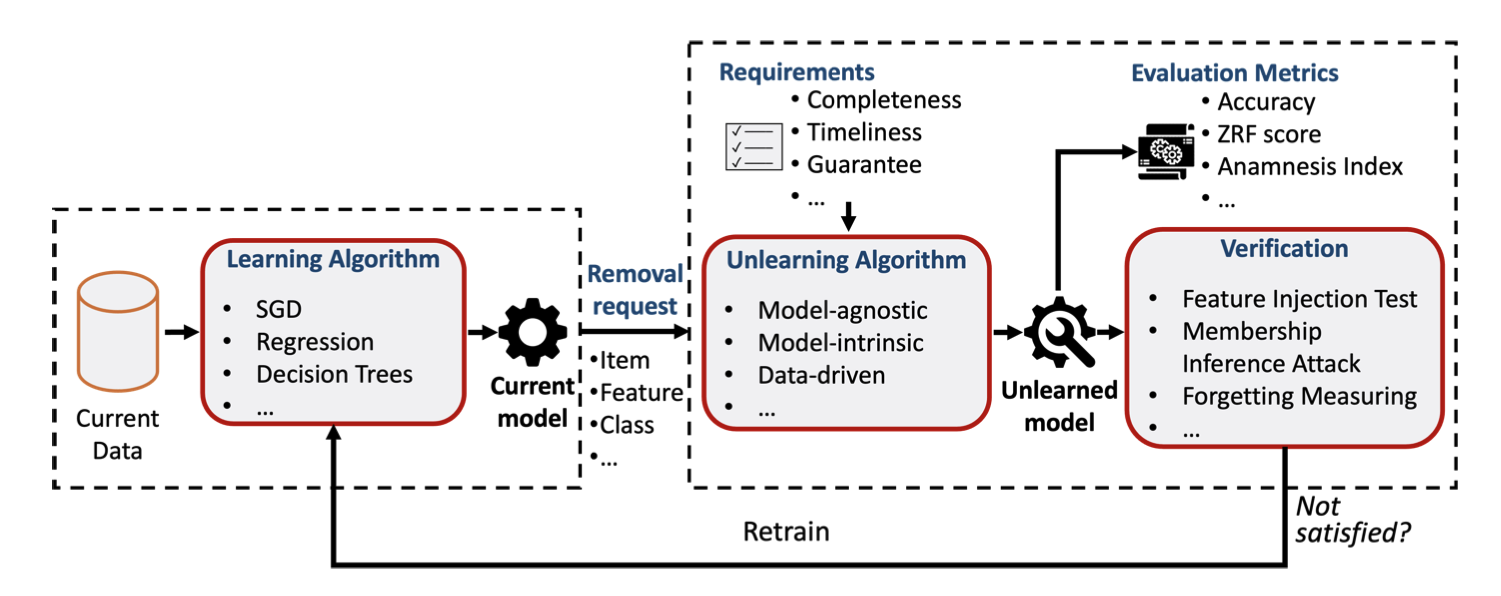
\includegraphics{assets/machine-unlearning-framework.png}

}

\caption{Machine Unlearning Framework}

\end{figure}%
\end{frame}

\begin{frame}{Formal Definition}
\phantomsection\label{formal-definition}
D = Dr+ Df

Df: forget set

Assumptions:

\begin{itemize}
\tightlist
\item
  The unlearning data are not big. Practically considering, also
  Otherwise, it is easier to do retraining.
\end{itemize}
\end{frame}

\begin{frame}{Retraining}
\phantomsection\label{retraining}
The problem makes unlearning difficult:

\begin{itemize}
\tightlist
\item
  Neural networks parameters do not tend to show any clear connection to
  the training data. AI models have to be considered as a whole.
\item
  Stochasticity and Incrementality of training
\item
  这种整体性很容易导致unlearning过头,catastrophic unlearning, reduce
  performance
\end{itemize}

\textbf{Retraining:}

\begin{itemize}
\tightlist
\item
  Delete target data and re-train the model with the rest of data from
  scratch
\item
  A naive way, but not always feasible
\item
  Achieves upper bound
\end{itemize}

The problem of retraining: - Doesn't worth, computation cost - Not
always having aceess to all training data
\end{frame}

\begin{frame}{Methodology}
\phantomsection\label{methodology}
Scenarios - Data Deletion - Class Removal

\begin{itemize}
\tightlist
\item
  Model-Agnostic or Model-Intrinsic
\item
  Data-Driven Approaches, most model-agnostic
\end{itemize}
\end{frame}

\begin{frame}{Method: SISA}
\phantomsection\label{method-sisa}
Data Partitioning (Efficient Retraining)

SISA (Sharded, Isolated, Sliced, Aggregated), 2021:

\begin{itemize}
\tightlist
\item
  Isolate: Isolate network and slice data into shards
\item
  build up correspondance bewteen divided network and data
\item
  Retraining the corresponding network of the data shard to be forgotten
\end{itemize}

Fractioning the retraining into smaller units
\end{frame}

\begin{frame}{Method: SISA}
\phantomsection\label{method-sisa-1}
\begin{figure}[H]

{\centering 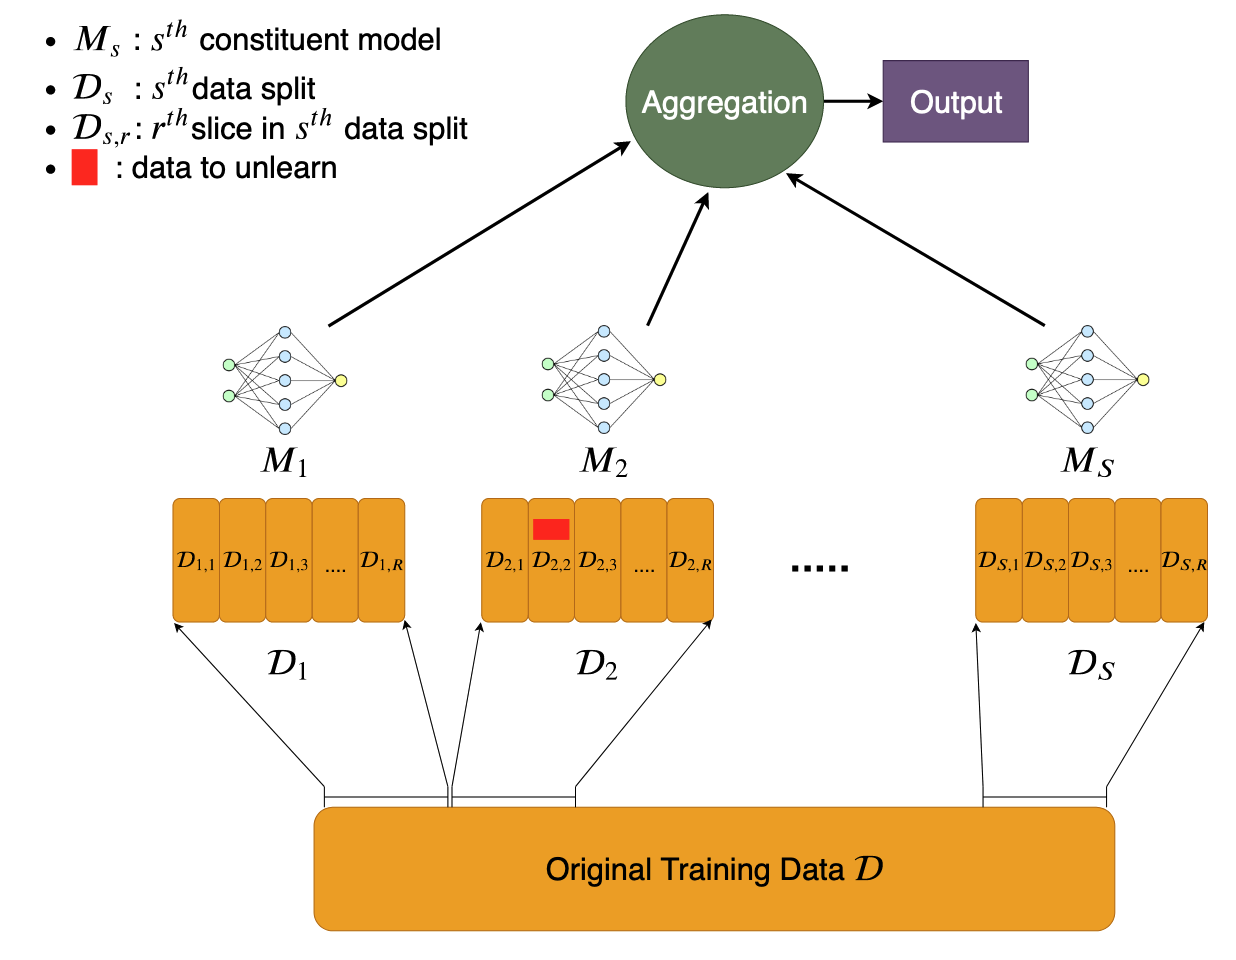
\includegraphics{assets/SISA.png}

}

\caption{SISA}

\end{figure}%
\end{frame}

\begin{frame}{SISA: Technical Details}
\phantomsection\label{sisa-technical-details}
\begin{itemize}
\tightlist
\item
  Slicing screenshots
\item
  Save the state of parameters of slices
\item
  Training: a) first locate the slice in which du is located, referred
  to as Dk,u, and (b) perform the training procedure as specified above
  from step u onwards using Dk,u \du; t
\item
  Aggregation: label-based majority vote
\end{itemize}
\end{frame}

\begin{frame}{Method: AmnesicML}
\phantomsection\label{method-amnesicml}
AmesicML, 2021: - would be to keep a record of each batch update.
However, if the data holder is only concerned about possible potential
removal of a subset of data, they need only keep the parameter updates
from batches containing that data. - we simply remove the parameter
updates from each batch

The problem: - The stochasticity and incremetaly of the training process
\end{frame}

\begin{frame}{Method: Error-Max Anti-sample generation}
\phantomsection\label{method-error-max-anti-sample-generation}
Error-Max Anti-sample generation - Class Removal - Max instead of Min
the loss - Do some repair

错误最大化噪声生成:这一步骤的核心是生成一个噪声矩阵,这个矩阵专门用于要遗忘的类别。通过原始模型学习这个噪声矩阵,噪声矩阵被设计来最大化模型在这个特定类别上的错误率,从而有效地干扰模型对这些类别的记忆。
2. 损害与修复步骤: •
损害(Impair)步骤:在这一步骤中,使用生成的噪声矩阵和非常高的学习速率对模型进行更新,以迅速减少模型对要遗忘的类别的记忆。这个过程类似于在模型的权重中注入噪声,破坏模型对特定数据的记忆。
•
修复(Repair)步骤:在损害步骤之后,模型的整体性能可能会受到影响。修复步骤通过在不包含要遗忘类别的数据上继续训练模型来恢复性能,修复因损害步骤而受损的其他功能。
\end{frame}

\begin{frame}[fragile]{Method: Linear Filteration}
\phantomsection\label{method-linear-filteration}
linear filtration, 2022

\begin{itemize}
\tightlist
\item
  Class Removal
\item
  应用过滤矩阵 F\_z 来直接修改模型的权重 W ,生成新的权重 W\_z ,
  不涉及新的数据训练或额外的学习步骤
\end{itemize}

Filter 的计算

\begin{enumerate}
\tightlist
\item
  计算预期预测: 对于每个类别 j ,计算该类的期望预测 \mathbf{a}\_j :
\end{enumerate}

\mathbf{a}\_j = \mathbb{E}{[}\mathbf{h}(\mathbf{x}) \textbar{} Y = j{]}

其中, \mathbf{h}(\mathbf{x}) 是分类器对输入 \mathbf{x} 的logits输出, Y
= j 表示数据点属于类别 j 。 2. 构建矩阵 A 和 B: • 矩阵 A
由所有类的期望预测组成,是一个 k \times k 矩阵:

A = {[}\mathbf{a}\_0 \textbar{} \mathbf{a}1 \textbar{} \cdots \textbar{}
\mathbf{a}{k-1}{]}

\begin{verbatim}
•   矩阵  B_z  由除了被遗忘类别外的类的变换预测构成,其中包含一个向量  z  替换被删除类别的向量:
\end{verbatim}

B\_z = {[}z \textbar{} \mathbf{a}1 \textbar{} \cdots \textbar{}
\mathbf{a}{k-1}{]}

\begin{verbatim}
3.  计算过滤矩阵  F_z :
\end{verbatim}

过滤矩阵 F\_z 是通过以下方式得到的,它将 A 转换为 B\_z :

F\_z = B\_z A\^{}\{-1\}

这个矩阵直接作用于原始的权重矩阵 W ,从而得到新的权重矩阵 W\_z :

W\_z = F\_z W

为什么是F\_z = B\_z A\^{}\{-1\}, 而不是 Bz 1. 计算预期预测:
对于每个类别 j ,计算该类的期望预测 \mathbf{a}\_j :

\mathbf{a}\_j = \mathbb{E}{[}\mathbf{h}(\mathbf{x}) \textbar{} Y = j{]}

其中, \mathbf{h}(\mathbf{x}) 是分类器对输入 \mathbf{x} 的logits输出, Y
= j 表示数据点属于类别 j 。 2. 构建矩阵 A 和 B: • 矩阵 A
由所有类的期望预测组成,是一个 k \times k 矩阵:

A = {[}\mathbf{a}\_0 \textbar{} \mathbf{a}1 \textbar{} \cdots \textbar{}
\mathbf{a}{k-1}{]}

\begin{verbatim}
•   矩阵  B_z  由除了被遗忘类别外的类的变换预测构成,其中包含一个向量  z  替换被删除类别的向量:
\end{verbatim}

B\_z = {[}z \textbar{} \mathbf{a}1 \textbar{} \cdots \textbar{}
\mathbf{a}{k-1}{]}

\begin{verbatim}
3.  计算过滤矩阵  F_z :
\end{verbatim}

过滤矩阵 F\_z 是通过以下方式得到的,它将 A 转换为 B\_z :

F\_z = B\_z A\^{}\{-1\}

这个矩阵直接作用于原始的权重矩阵 W ,从而得到新的权重矩阵 W\_z :

W\_z = F\_z W
\end{frame}

\section{Continual Learning + Machine
Unlearning}\label{continual-learning-machine-unlearning}

\begin{frame}{How Continual Learning + Machine Unlearning?}
\phantomsection\label{how-continual-learning-machine-unlearning}
In essence, Continual learning is a non-stationary data stream.

What's the point?

\begin{itemize}
\tightlist
\item
  Provide unlearning options only for this scheme. Less meaningful
\item
  Good for continual learning itself:

  \begin{itemize}
  \tightlist
  \item
    Promote network capacity? (really? investigate MU methods) Take it
    as a manual approach to balance S-P trade-off
  \end{itemize}
\end{itemize}
\end{frame}

\begin{frame}{We do have proposed paradigms, though.}
\phantomsection\label{we-do-have-proposed-paradigms-though.}
我找到了两篇类似的把unlearning往CL靠的论文,造了两个不一样的场景:
\end{frame}

\begin{frame}{Proposed Paradigm: LSF Problem}
\phantomsection\label{proposed-paradigm-lsf-problem}
CLPU:
https://lifelong-ml.cc/Conferences/2022/acceptedpapersandvideos/conf-2022-44

CLPU是在以任务为单位的,task-level,什么时候忘是根据指示,例如训练完任务1,可能在任务2,3,4训练完的时候要求1忘,也可以永远不要求

CLPU的目标是在没要求忘的任务效果尽量好(CL本身的目标),并且要求1.
训了要求忘的任务然后忘掉的结果,尽量和2.要求忘的任务从来没存在过训练的结果
尽量一致(unlearning 的目标) Df a task as the forgetting unit

At the k-th task, we are given the dataset Dk and the preservation set
CP k . We use index k for the new task and p for the previous tasks.
Definition 1 (LSF Problem). The Learning with Selective Forgetting (LSF)
problem is defined as follows: • Objective: Learn a model fθ : X → Y.
This model fθ should map a test input x to its correct class label y if
x is in the preservation set CP . Otherwise, fθ should map x to a wrong
class label y′ 6= y. • Constraint: No original samples or generative
models for the past tasks are available after the new task begins.
\end{frame}

\begin{frame}{Proposed Paradigm: LSF Problem}
\phantomsection\label{proposed-paradigm-lsf-problem-1}
explains that this requires users to explicitly define which tasks will
be learned permanently and which tasks will be learned only temporarily.

Sequence tasks Sequence Requests inserted tasks, R,T,F (by assumption in
CLPU paper) Should be R,F??
\end{frame}

\begin{frame}{}
\phantomsection\label{section}
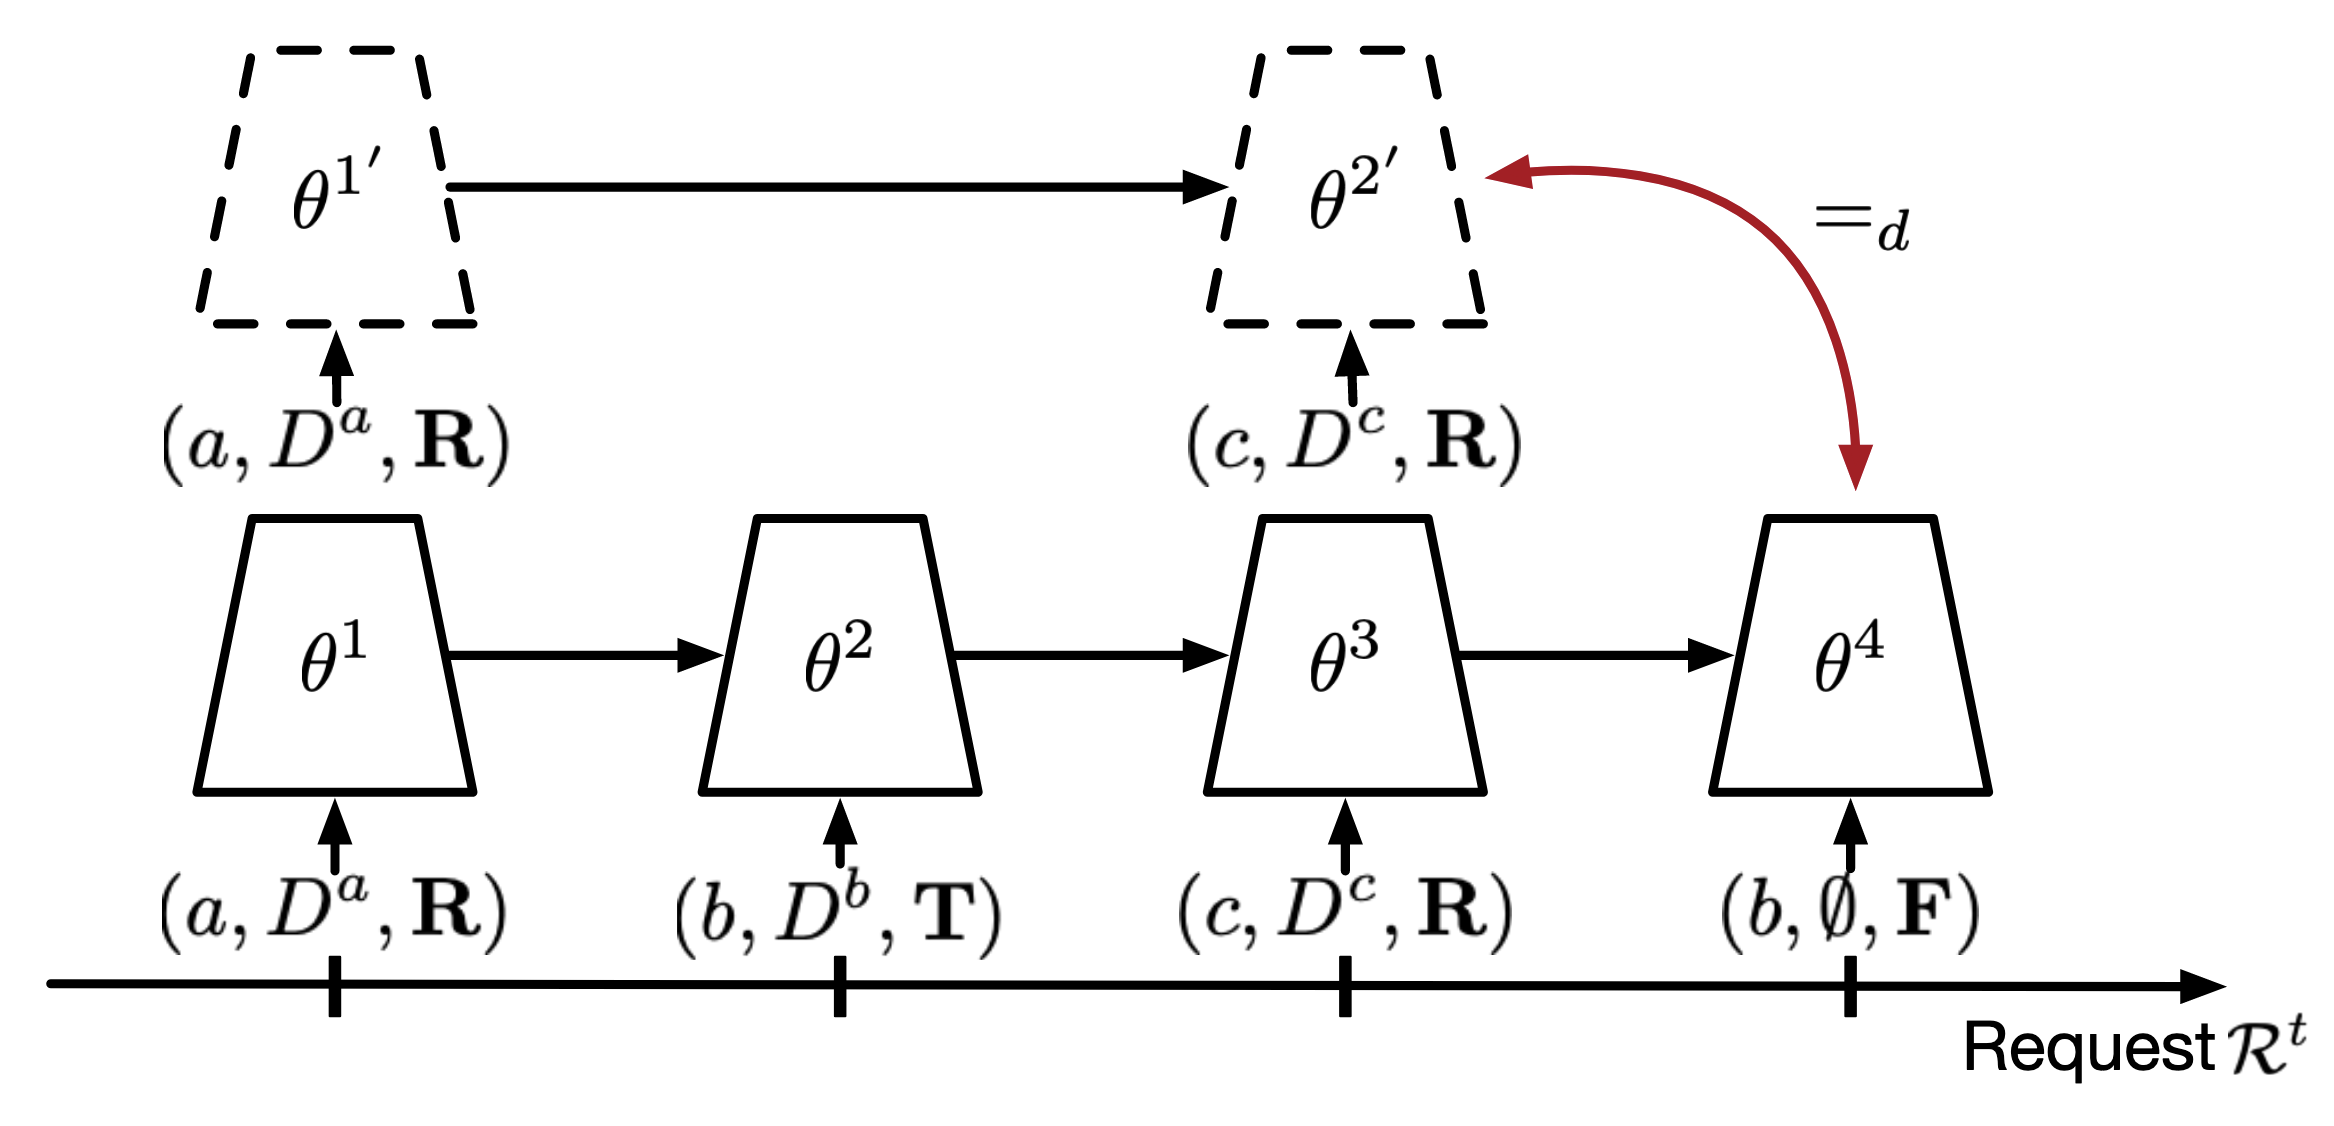
\includegraphics{ssets/CLPU.png}
\end{frame}

\begin{frame}{Metrics}
\phantomsection\label{metrics}
\end{frame}

\begin{frame}{CLPU DER++}
\phantomsection\label{clpu-der}
A naive method:

\begin{itemize}
\tightlist
\item
  Take isolated for potential task to be forgetted.
\item
  Use R, T. setback, have to know if it can be forgetted. Should develop
  forget at any time.
\item
\end{itemize}
\end{frame}

\begin{frame}{Selective Forgetting}
\phantomsection\label{selective-forgetting}
LSF: https://www.ijcai.org/proceedings/2021/137

LSF
是在每个任务要求一部分类别是要unlearn的,class-level,每次训练新任务时都要求前面任务的unlearn
set开始忘
LSF的目标是每个任务里没要求忘的类的数据效果尽量好(CL本身的目标),并且要求忘的数据效果下降的尽量厉害(unlearning
的目标)。这个目标是为了忘而忘

To the best of our knowledge, only one previous paper discusses a
similar problem setting pertaining to selective forgetting in continual
learning (Shibata et al., 2021). However, the problem in that paper is
different from CLPU as it defines forgetting as maximally degrading the
performance on a task. As discussed in Sec. 5, this requirement is not
privacy-preserving and can potentially leak information (e.g., that the
task has been previously learned).

\begin{itemize}
\tightlist
\item
\end{itemize}
\end{frame}

\section{Next Step}\label{next-step}

\begin{frame}{Thinking}
\phantomsection\label{thinking}
\begin{enumerate}
\tightlist
\item
  这些工作只是讨论在CL框架下搞unlearning而已,我认为单纯这样做没什么意义。
\item
  我认为unlearning对continual learning本身是好处(例如释放network
  capacity),
\item
  虽然他们指标里带着CL本身的目标,但是没有体现出来
\end{enumerate}

\begin{itemize}
\tightlist
\item
  CL本身的目标就是在没要求忘的任务上效果好。这些工作会把带unlearning的和不带的普通的CL
  baseline(如EWC)进行比较,其中不带unlearning的方法就把所有任务不管要不要unlearn都一起学,然后只算没要求unlearn的任务上的平均准确率。按说,如果把所有的一起学了,肯定会挤占网络资源,导致效果不好,如果unlearning这个行为可以释放资源的话,带unlearning的算法效果应该更好的,但这个论文里的结果表格好像还不如。\\
\item
  我猜是没有达到network
  capacity的极限,不需要释放capacity,即使unlearning有释放capacity的作用,也不会对效果有好的贡献。你看论文里比较的方法都是允许不够的时候向外面要capacity的,就是说capacity不是fixed而是可以扩张的,他们可以在缺的时候直接用扩张要到,不需要unlearning去释放。
\end{itemize}

the forgotten data has to be known a priori when the original model is
trained {[}45{]}. 4. 所以要和解决network
capacity问题这件事搭边,得放在不允许扩张的方法里面试,比如HAT,这样unlearning释放capacity然后让效果变好的作用就能体现出来了。论文里可以说既能系统性解决network
capacity不足的问题,也能有效unlearning。
\end{frame}

\begin{frame}{next step}
\phantomsection\label{next-step-1}
\begin{itemize}
\tightlist
\item
  明确目标,是unlearning的目标,还是为了持续学习好

  \begin{itemize}
  \tightlist
  \item
    调查MU的方法
  \item
    To design a new CL MU algorithm promoting network capacity.
  \end{itemize}
\item
  To validate, Compare the 1,2,3,F2,4,F3\ldots{} fixed network average
  1,2,3,4 and 1,4 after forgetting 2,3
\end{itemize}

也可以沿着他们提的这个场景去解决他们的问题,但我不看好,
它们造的。LSF场景感觉没什么意义,它忘的时候不是由我们说了算的;CLPU其实仔细看它们有个限定,它区分R和T,有的任务(标记为R的)会提前知道它之后永远不会被要求忘掉,也是个非常特殊的场景。我感觉是为了写论文或者套他们的想法方便硬造的特殊场景,没用通用性,而且指标很复杂。
\end{frame}

\begin{frame}{Thank You}
\phantomsection\label{thank-you}
\centering \Large

Thank you for your attention!

\hfill\break

Please feel free to ask any questions or reach out to me at:

\url{wangpengxiang@stu.pku.edu.cn}

\vfill

\begin{figure}
  \centering
  \begin{subfigure}{0.2\textwidth}
    \centering
    
\includegraphics[height=0.8cm]{../assets/pku-logo.png}
  \end{subfigure}
  \hspace{0.5cm}
  \begin{subfigure}{0.2\textwidth}
    \centering
    
\includegraphics[height=0.8cm]{../assets/uob-logo.png}
  \end{subfigure}
\end{figure}
\end{frame}




\end{document}
